\chapter{Hellinger Based Distance for Uncertain time series}
\label{helinger}
Deterministic Measures like traditional similarity measures, return a real number as
the distance between two uncertain time series. 
\section{DUST}
\cite{murthy2013generalized} is the only
deterministic similarity measure defined for uncertain time series. Given two uncertain time series $X=<X_1, \ldots,X_n>$ and $Y=<Y_1, \ldots,Y_n>$ , the distance between
two uncertain values $X_i$, $Y_i$ is defined as the distance between their true (unknown) values
r($X_i$), r($Y_i$): $dist(X_i, Y_i) = |r(X_i) - r(Y_i)|$. This distance is used to measures the
similarity of two uncertain values. $\varphi(|X_{i}-Y_{i}|)$ is the probability that the reals values at timestamp i are equal, given
the observed values at that timestamp i.e.
\begin{eqnarray}
\varphi(|X_{i}-Y_{i}|)=Pr(dist(0|r(X_{i})-r(Y_{i})|=0).
\end{eqnarray}
This similarity function is then used inside the dust dissimilarity function:
\begin{eqnarray}
dust(X_{i},Y_{i})=\sqrt{-log(\varphi(|X_{i}-Y_{i}|))+log(\varphi(0))}.
\end{eqnarray}
The distance between uncertain time series $X=<X_1, \ldots,X_n>$ and\\ $Y=<Y_1, \ldots,Y_n>$ in DUST
is then defined as follows:
\begin{eqnarray}
DUST(X,Y)=\sqrt{\stackrel[i=1]{n}{\sum}dust(X_{i},Y_{i})^{^{2}}}.
\end{eqnarray} 
The disadvantage of DUST is that it  breaks the triangle inequality for small distances. Triangular inequality is a desirable property of dissimilarity functions because it makes it possible to speed-up the comparison of time series. For example, for density based clustering two time series A and B are considered similar if the distance between them is less than $\epsilon$. Thus, if the sum of the distances d (A, B) and d (B, C) is less than $\epsilon$, we deduce that the distance d (A, C) is also without calculating it. The triangular inequality is also used for the exact indexing of time series \cite{keogh2001locally}.


To remedy this, we introduce a new deterministic distance function based on the
Hellinger distance that evaluate the dissimilarity between uncertain time series and respects triangular
inequality.

\section{Hellinger Based Distance}
To evaluate the similarity between two probability distributions, we can measure the area of intersection between these two probability distributions (Figure \ref{Bhattacharyya}) . If the area of this intersection is zero, then the probability distributions are disjoint, if it is 1 then the probability distributions are identical. The area of this intersection can be calculated using the Bhattacharyya coefficient (B) \cite{patra2015new}.

\begin{figure}
\centering
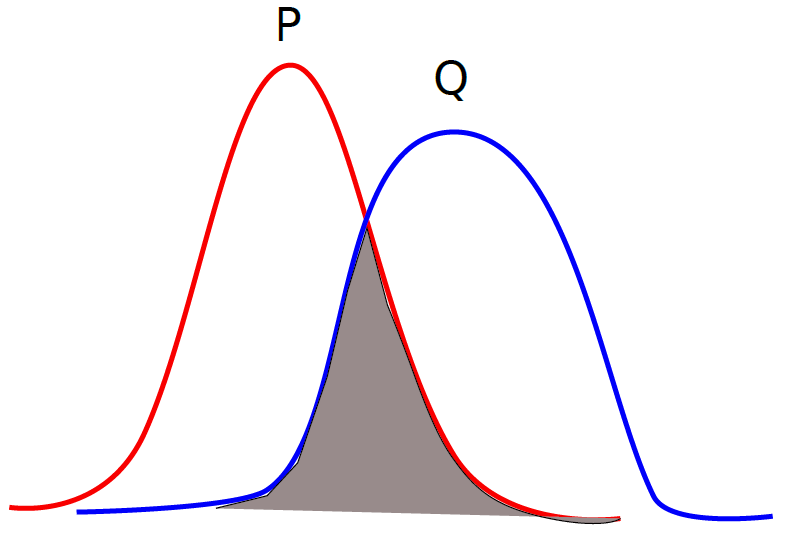
\includegraphics[scale=0.4]{images/bhattacharyya}
\caption{Bhattacharyya}
\label{Bhattacharyya}

\end{figure}

The \textbf{Hellinger} distance, based on the use of the Bhattacharyya coefficient, allows to measure the dissimilarity between two probability distributions. It is defined as follows:

\begin{definition}
The Hellinger distance between two  probability measures  $P$ and $Q$ that are absolutely
continuous relative to some $\sigma$-finite measure $\mu$ on a measurable space $(x,\beta)$ is defined
by the formula:
\begin{eqnarray}
H(P,Q)=\{2[1-B(P,Q)]\}^{\frac{1}{2}},
\end{eqnarray}
where
\begin{eqnarray}
B(P,Q)=\int\sqrt{\frac{dP}{d\mu}}\sqrt{\frac{dQ}{d\mu}}d\mu.
\end{eqnarray}
\end{definition}

\begin{theorem}
\label{hellinger}
The Hellinger distance satisfy the triangle inequality\\ \cite{ibragimov2013statistical}.
\end{theorem}

Based on Hellinger distance we define the HBD distance (Hellinger Based Distance) which measures the dissimilarity between two uncertain time series:

\begin{definition}
The distance between uncertain time series $X=<X_1, \ldots,X_n>$ and $Y=<Y_1, \ldots,Y_n>$ under
Hellinger Based Distance is then defined as follows:
\begin{eqnarray}
HBD(X,Y)=\sqrt{\stackrel[i=1]{n}{\sum}H(X_{i},Y_{i})^{^{2}}}.
\end{eqnarray} 
\end{definition}

\begin{theorem}
HBD distance satisfy the triangle inequality.
\end{theorem}

\begin{proof}
Let $X=<X_1, \ldots,X_n>$, $Y=<Y_1, \ldots,Y_n>$, $Z=<Z_1, \ldots,Z_n>$ be three uncertain time series, we want to proof that

\begin{eqnarray}
\sqrt{\stackrel[i=1]{n}{\sum}H(X_{i},Y_{i})^{^{2}}}
+
\sqrt{\stackrel[i=1]{n}{\sum}H(Y_{i},Z_{i})^{^{2}}}
\geq
\sqrt{\stackrel[i=1]{n}{\sum}H(X_{i},Z_{i})^{^{2}}}.
\end{eqnarray} 


First, let us show that:
\begin{eqnarray}
\left( \sqrt{\stackrel[i=1]{n}{\sum}H(X_{i},Y_{i})^{^{2}} }\right)
\times
\left( \sqrt{\stackrel[i=1]{n}{\sum}H(Y_{i},Z_{i})^{^{2}}} \right)
\geq
\stackrel[i=1]{n}{\sum}H(X_{i},Y_{i})H(Y_{i},Z_{i})
\label{eq1}
\end{eqnarray}
by squaring the two members of the inequality (\ref{eq1}) we obtain

\begin{eqnarray}
\left( \stackrel[i=1]{n}{\sum}H(X_{i},Y_{i})^{^{2}} \right)
\times
\left( \stackrel[i=1]{n}{\sum}H(Y_{i},Z_{i})^{^{2}} \right)
\geq
\left( \stackrel[i=1]{n}{\sum}H(X_{i},Y_{i})H(Y_{i},Z_{i}) \right)^2
\end{eqnarray}

\begin{eqnarray}
i.e.
\left( \stackrel[i=1]{n}{\sum}H(X_{i},Y_{i})^{^{2}} \right)
\times
\left( \stackrel[i=1]{n}{\sum}H(Y_{i},Z_{i})^{^{2}} \right) \\
-
\left( \stackrel[i=1]{n}{\sum}H(X_{i},Y_{i})H(Y_{i},Z_{i}) \right)^2
\geq
0
\label{eq2}
\end{eqnarray}
by developing and reducing the expression(\ref{eq2}), we obtain

\begin{eqnarray}
i.e.
\underset{i,j\epsilon\{1,...,k\}\,and\,i\neq j}{\sum}\left(H(X_{i},Y_{i})-H(Y_{j},Z_{j})\right)^{2}
\geq
0
\end{eqnarray}
This shows that the inequality (\ref{eq1}) is true.
Let us now show that HBD satisfies the triangular inequality : 
according to Theorem \ref{hellinger}, 
\begin{eqnarray}
H(X_{i},Y_{i})+H(Y_{i},Z_{i})\geq H(X_{i},Z_{i})
\end{eqnarray}
By squaring the two members of the inequality, we obtain
\begin{eqnarray}
H(X_{i},Y_{i})^2+H(Y_{i},Z_{i})^2 + 2H(X_i, Y_i)H(Y_i, Z_i)\geq
H(X_{i},Z_{i})^2.
\end{eqnarray}

\begin{eqnarray}
i.e.
\stackrel[i=1]{n}{\sum}H(X_{i},Y_{i})^2+\stackrel[i=1]{n}{\sum}H(Y_{i},Z_{i})^2
+ 2\stackrel[i=1]{n}{\sum}H(X_i, Y_i)H(Y_i, Z_i) \\ \geq
\stackrel[i=1]{n}{\sum}H(X_{i},Z_{i})^2.
\end{eqnarray}

according to inequality \ref{eq1}, we obtain
\begin{eqnarray}
\stackrel[i=1]{n}{\sum}H(X_{i},Y_{i})^2+\stackrel[i=1]{n}{\sum}H(Y_{i},Z_{i})^2 \\
+ 2\left( \sqrt{\stackrel[i=1]{n}{\sum}H(X_{i},Y_{i})^{^{2}} }\right)
\times
\left( \sqrt{\stackrel[i=1]{n}{\sum}H(Y_{i},Z_{i})^{^{2}}} \right)
\geq
\stackrel[i=1]{n}{\sum}H(X_{i},Z_{i})^2.
\end{eqnarray}

\begin{eqnarray}
i.e.
\left( \sqrt{\stackrel[i=1]{n}{\sum}H(X_{i},Y_{i})^{^{2}} }
+
\sqrt{\stackrel[i=1]{n}{\sum}H(Y_{i},Z_{i})^{^{2}}} \right)^2
\geq
\stackrel[i=1]{n}{\sum}H(X_{i},Z_{i})^2.
\end{eqnarray}

\begin{eqnarray}
i.e.
 \sqrt{\stackrel[i=1]{n}{\sum}H(X_{i},Y_{i})^{^{2}} }
+
\sqrt{\stackrel[i=1]{n}{\sum}H(Y_{i},Z_{i})^{^{2}}}
\geq
\sqrt{\stackrel[i=1]{n}{\sum}H(X_{i},Z_{i})^2}.
\end{eqnarray}
This is what had to be demonstrated
\end{proof}

The problem with the deterministic uncertain distance distances DUST and HBD is that their expression varies as a function of the probability law that uncertainty follows. Their use therefore requires knowledge of the law of probability of the uncertainty 
contained in the data, which is not always possible in practice.






































